\documentclass[aspectratio=169, usenames, dvipsnames]{beamer}

\usetheme{Pittsburgh}

\usepackage[utf8]{inputenc}
\usepackage{amsmath}
\usepackage{amsfonts}
\usepackage{amssymb}
\usepackage{graphicx}
\usepackage{multicol}
\usepackage{hyperref}
\usepackage{framed}
\usepackage{tikz}
\usetikzlibrary{shapes,arrows}
\usepackage{xspace}                     % Correct spacings
\usepackage{csquotes} 
\usepackage{stex-logo}
\usepackage{lmodern}

\usepackage{tkz-kiviat}

\beamertemplatenavigationsymbolsempty 
\setbeamertemplate{footline}[frame number]

\newcommand{\MMT}{\textsf{MMT}\xspace}
\newcommand{\OMDOC}{\textsf{OMDoc}\xspace}
\def\ALeA{\textsc{ALeA}\xspace}

\author{Jonas Betzendahl and Michael Kohlhase and Dennis Müller}
\title{Guided Tours in \ALeA}
\subtitle{Assembling Tailored Educational Dialogues from Semantically Annotated Learning Objects}

\begin{document}

%------------------------------------------------------------------------------------
\begin{frame}
\begin{center}
\huge \textbf{Guided Tours in \ALeA}\medskip

\large Assembling Tailored Educational Dialogues\\ from Semantically Annotated Learning Objects

\normalsize 
\bigskip\bigskip

\large \emph{Jonas Betzendahl}, Michael Kohlhase, Dennis Müller\\
\texttt{[firstname].[lastname]@fau.de}\bigskip

\small
AI4AI Workshop @ ECAI23\\
2023 -- 10 -- 01
\medskip


\includegraphics[scale=0.5]{images/fau_logo.png}
\qquad

\includegraphics[scale=0.25]{images/kwarclogo_faublau.png} 
\end{center}
\end{frame}

\section{Introduction}

\begin{frame}
\frametitle{Motivation}
\end{frame}

\begin{frame}[fragile]
\frametitle{Context: \ALeA}

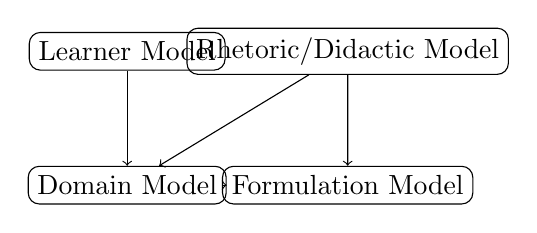
\begin{tikzpicture}[xscale=2.8,yscale=1.7]
  \node[draw,rounded corners] (dm) at (0,0) {Domain Model};
  \node[draw,rounded corners] (lm) at (0,1) {Learner Model};
  \node[draw,rounded corners] (fm) at (1,0) {Formulation Model};
  \node[draw,rounded corners] (im) at (1,1) {Rhetoric/Didactic Model};
  \draw[->] (lm) -- (dm);
  \draw[->] (fm) -- (dm);
  \draw[->] (im) -- (dm);
  \draw[->] (im) -- (fm);
\end{tikzpicture}
\end{frame}

\begin{frame}
\frametitle{\sTeX}
\begin{center}
Semantic annotation on the \emph{concept level} in course materials.\bigskip

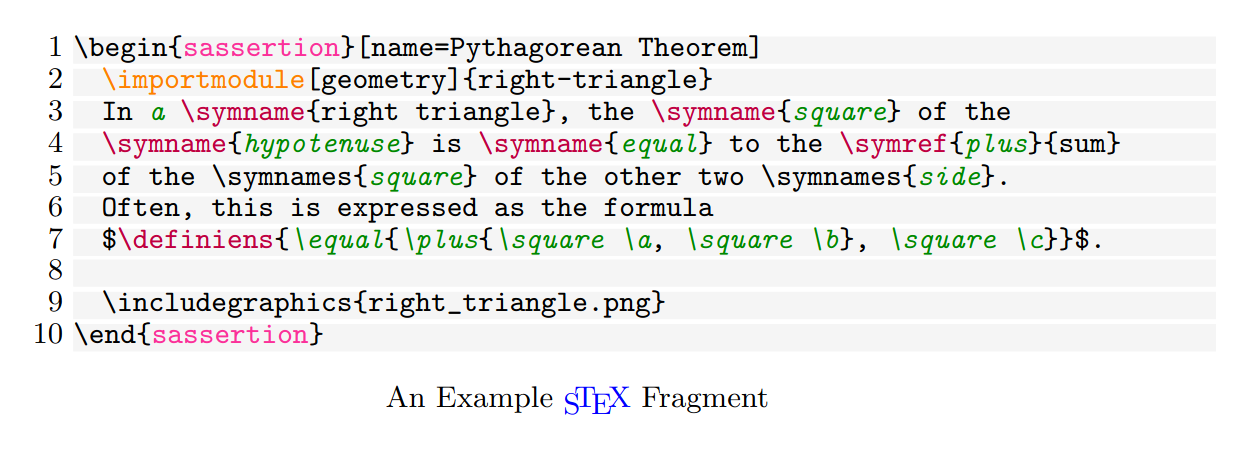
\includegraphics[width=0.95\textwidth, keepaspectratio]{images/stex_example.png} 
\end{center}
\end{frame}

\begin{frame}[fragile]
\frametitle{The Learner Model}
\begin{minipage}{0.4\textwidth}
foo bar
\end{minipage}%
\begin{minipage}{0.6\textwidth}
\begin{tikzpicture}[rotate=-35, scale=0.5]
\tkzKiviatDiagram[label space = 1.5]{Remember,Understand,Apply,Analyse,Evaluate,Create}
\tkzKiviatLine[thick,color=red](7.25,5.5,4,6.5,7,2)
\tkzKiviatLine[thick,color=blue](3,9,6,5.2,5.6,4.8)
\tkzKiviatLine[thick,color=green](5.9,6.1,3,3,2.3,9.2)
\end{tikzpicture}
\end{minipage}%
\end{frame}

\section{The Algorithm}

\begin{frame}
\frametitle{Educational Dialogues}
\begin{minipage}{0.4\textwidth}
Educational Dialogues good!
\end{minipage}%
\begin{minipage}{0.6\textwidth}
\pause
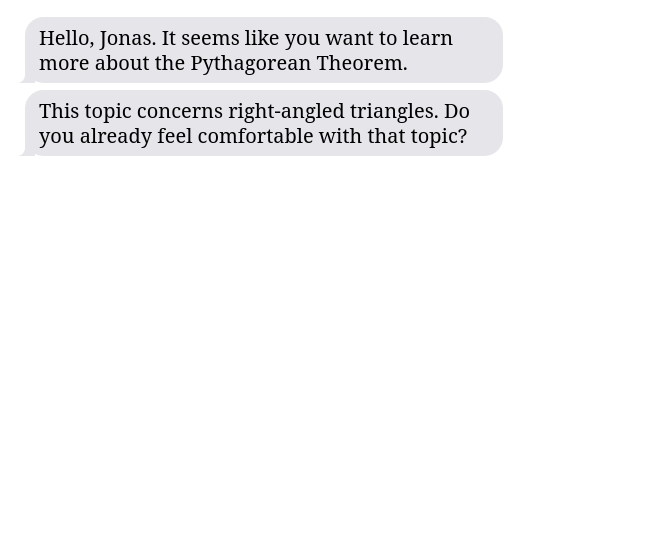
\includegraphics[height=0.75\textheight,keepaspectratio]{images/bubbles_example_step1} 
\end{minipage}%
\end{frame}

\begin{frame}
\frametitle{Educational Dialogues}
\begin{minipage}{0.4\textwidth}
Educational Dialogues good!
\end{minipage}%
\begin{minipage}{0.6\textwidth}
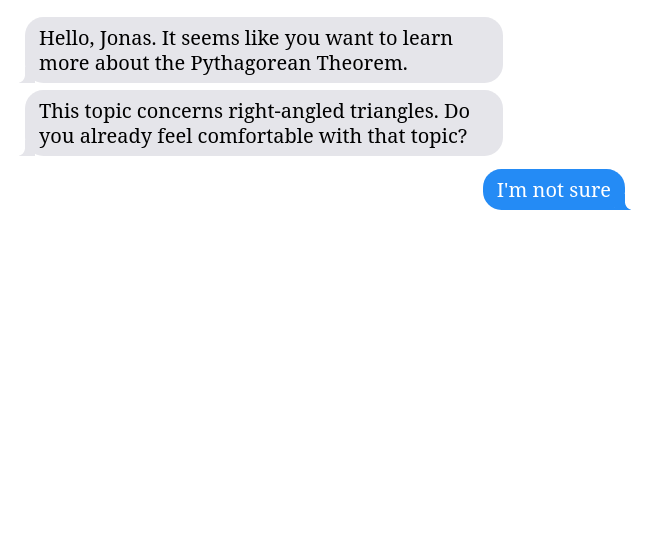
\includegraphics[height=0.75\textheight,keepaspectratio]{images/bubbles_example_step2} 
\end{minipage}%
\end{frame}

\begin{frame}
\frametitle{Educational Dialogues}
\begin{minipage}{0.4\textwidth}
Educational Dialogues good!
\end{minipage}%
\begin{minipage}{0.6\textwidth}
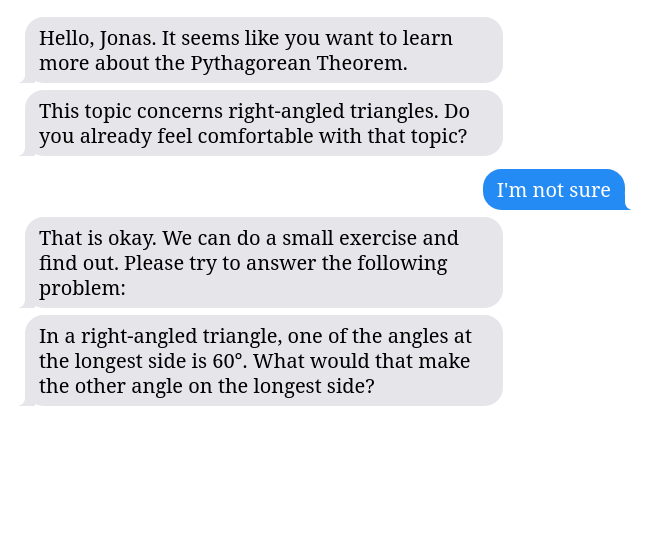
\includegraphics[height=0.75\textheight,keepaspectratio]{images/bubbles_example_step3} 
\end{minipage}%
\end{frame}

\begin{frame}
\frametitle{Educational Dialogues}
\begin{minipage}{0.4\textwidth}
Educational Dialogues good!
\end{minipage}%
\begin{minipage}{0.6\textwidth}
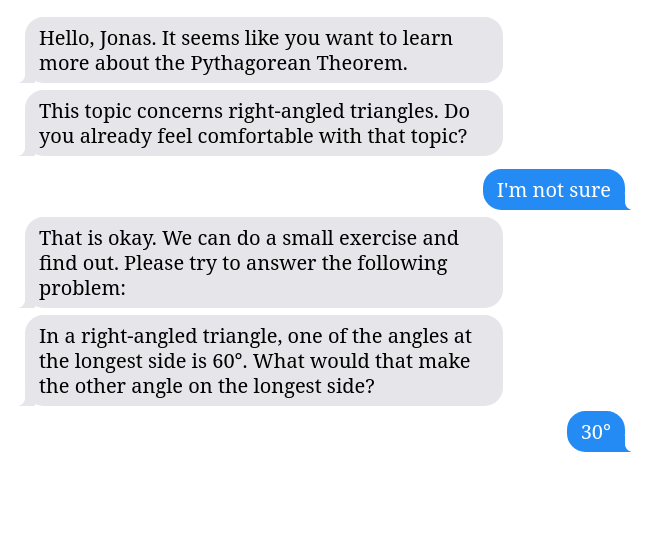
\includegraphics[height=0.75\textheight,keepaspectratio]{images/bubbles_example_step4} 
\end{minipage}%
\end{frame}

\begin{frame}
\frametitle{Educational Dialogues}
\begin{minipage}{0.4\textwidth}
Educational Dialogues good!
\end{minipage}%
\begin{minipage}{0.6\textwidth}
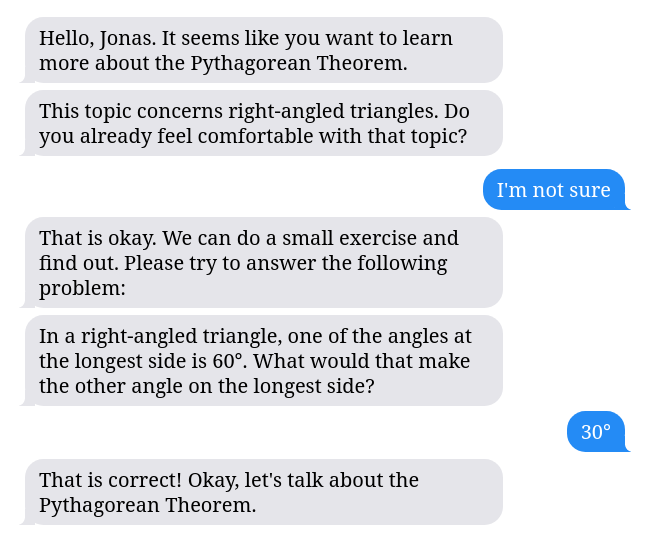
\includegraphics[height=0.75\textheight,keepaspectratio]{images/bubbles_example_step5} 
\end{minipage}%
\end{frame}

\begin{frame}
\frametitle{Overview}
\begin{minipage}{0.7\textwidth}
\vspace*{-10px}
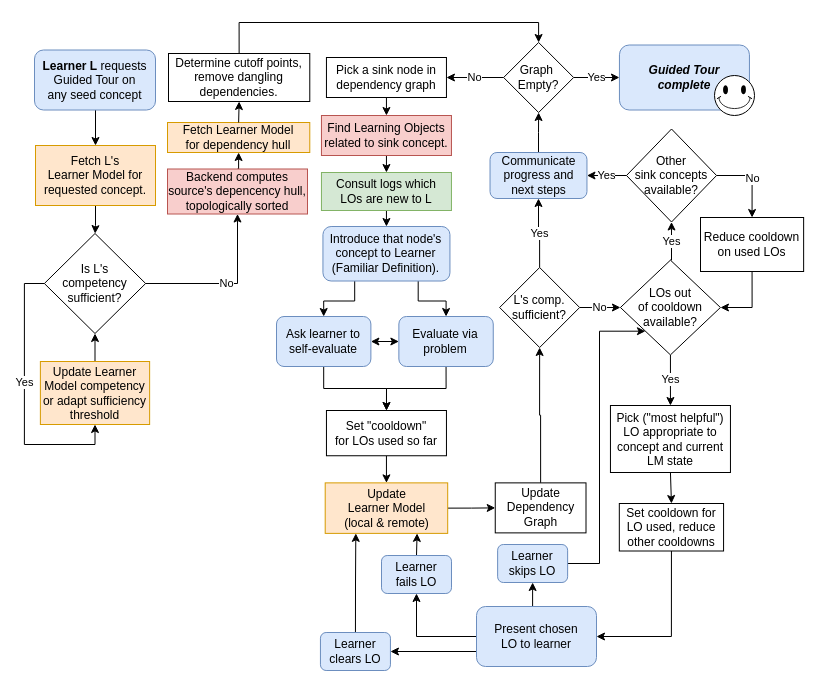
\includegraphics[height=0.9\textheight,keepaspectratio]{images/gt_algorithm_square}
\end{minipage}%
\begin{minipage}{0.3\textwidth}
The complete algorithm for guided tours in \ALeA.
\end{minipage}%
\end{frame}

\begin{frame}
\frametitle{Initialisation}
\begin{minipage}{0.7\textwidth}
\vspace*{-10px}
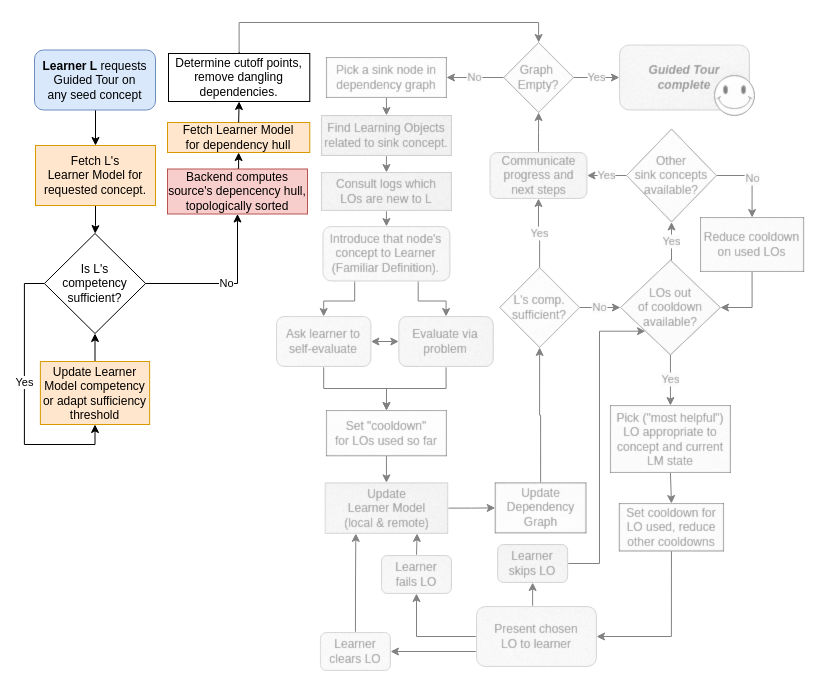
\includegraphics[height=0.9\textheight,keepaspectratio]{images/gt_algorithm_square_step1}
\end{minipage}%
\begin{minipage}{0.3\textwidth}
\end{minipage}%
\end{frame}

\begin{frame}
\frametitle{Concept Introduction}
\begin{minipage}{0.7\textwidth}
\vspace*{-10px}
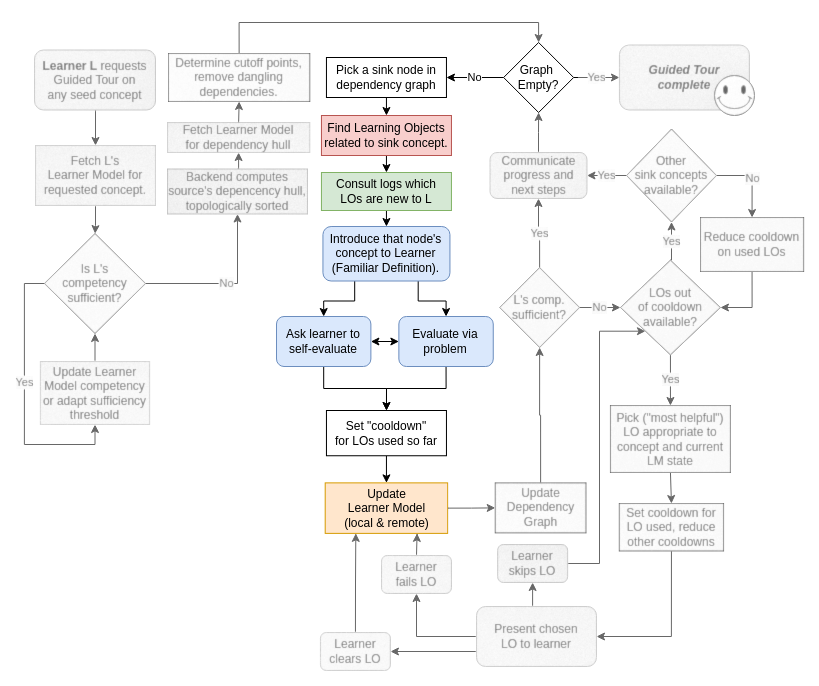
\includegraphics[height=0.9\textheight,keepaspectratio]{images/gt_algorithm_square_step2}
\end{minipage}%
\begin{minipage}{0.3\textwidth}
\end{minipage}%
\end{frame}

\begin{frame}
\frametitle{Learning}
\begin{minipage}{0.7\textwidth}
\vspace*{-10px}
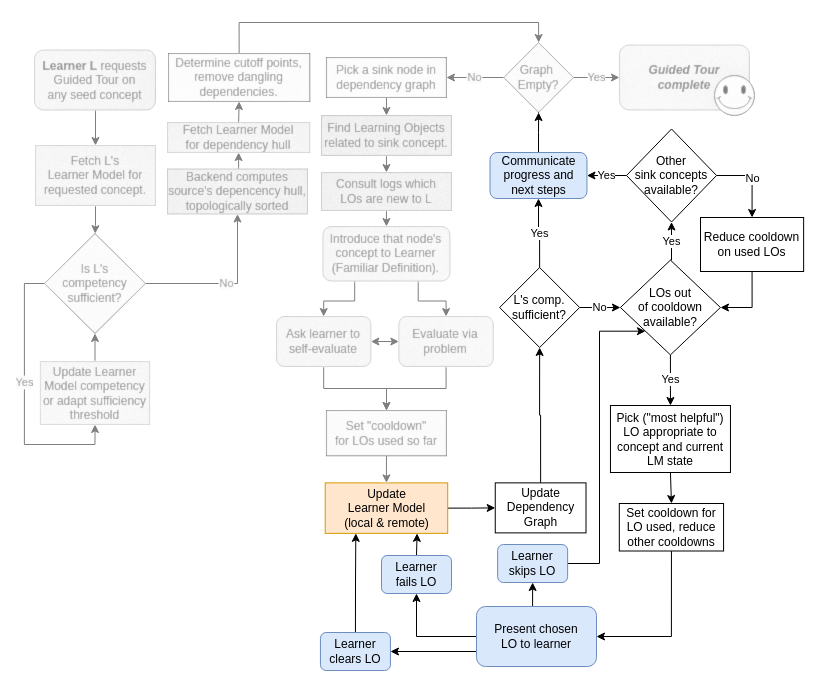
\includegraphics[height=0.9\textheight,keepaspectratio]{images/gt_algorithm_square_step3}
\end{minipage}%
\begin{minipage}{0.3\textwidth}
\end{minipage}%
\end{frame}

\begin{frame}
\frametitle{Finish}
\begin{minipage}{0.7\textwidth}
\vspace*{-10px}
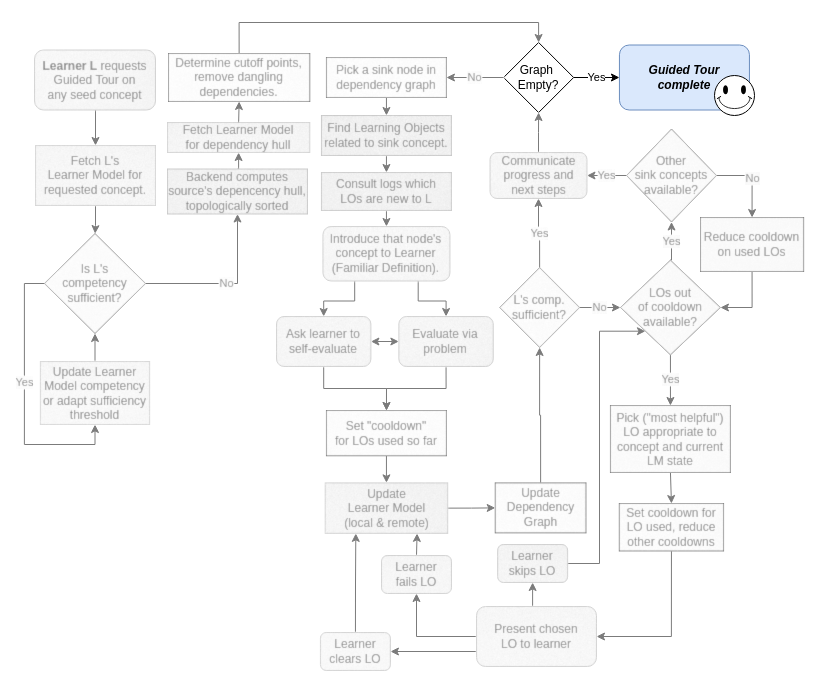
\includegraphics[height=0.9\textheight,keepaspectratio]{images/gt_algorithm_square_step4}
\end{minipage}%
\begin{minipage}{0.3\textwidth}
\end{minipage}%
\end{frame}

\begin{frame}
\frametitle{Recap}
\begin{minipage}{0.7\textwidth}
\vspace*{-10px}
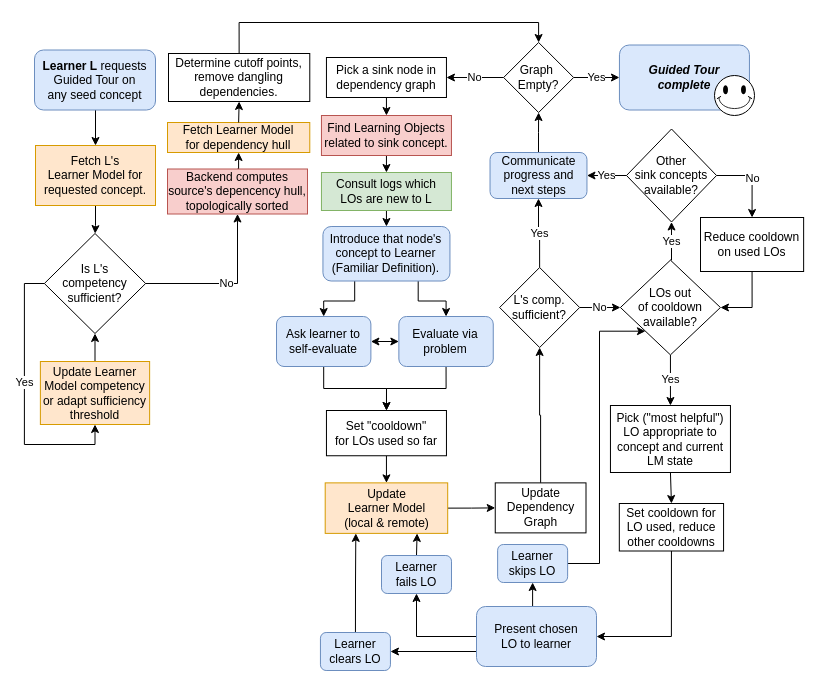
\includegraphics[height=0.9\textheight,keepaspectratio]{images/gt_algorithm_square}
\end{minipage}%
\begin{minipage}{0.3\textwidth}
The complete algorithm for guided tours in \ALeA.
\end{minipage}%
\end{frame}

\section{Wrap-up}

\end{document}